\documentclass[12pt,a4paper]{article}

% Packages
\usepackage[utf8]{inputenc}
\usepackage[T1]{fontenc}
\usepackage[english]{babel}
\usepackage{geometry}
\usepackage{hyperref}
\usepackage{graphicx}
\usepackage{amsmath}
\usepackage{amssymb}
\usepackage{booktabs}
\usepackage{longtable}
\usepackage{array}
\usepackage{xcolor}
\usepackage{fancyhdr}
\usepackage{listings}
\usepackage{caption}
\usepackage{subcaption}
\usepackage{titlesec}
\usepackage{tocloft}
\usepackage{enumitem}
\usepackage{float}
\usepackage{microtype}
\usepackage{setspace}
\usepackage{abstract}
\usepackage{tikz}
\usetikzlibrary{shapes.geometric, arrows.meta, positioning, fit, backgrounds}

% Page geometry
\geometry{
  a4paper,
  top=2.5cm, bottom=2.5cm,
  left=2.5cm, right=2.5cm
}

% Colors
\definecolor{phantomred}{RGB}{200, 30, 30}
\definecolor{codebg}{RGB}{245, 245, 245}
\definecolor{codeframe}{RGB}{180, 180, 180}
\definecolor{criticalred}{RGB}{200, 0, 0}
\definecolor{highorange}{RGB}{220, 100, 0}
\definecolor{mediumyellow}{RGB}{180, 140, 0}
\definecolor{lowgreen}{RGB}{30, 140, 30}

% Hyperref setup
\hypersetup{
  colorlinks=true,
  linkcolor=phantomred,
  urlcolor=blue,
  citecolor=black,
  pdftitle={Phantom: An Autonomous AI-Driven Penetration Testing Agent},
  pdfauthor={Gadouri Redwan},
  pdfsubject={Autonomous AI Security Agent},
}

% Header/Footer
\pagestyle{fancy}
\fancyhf{}
\fancyhead[L]{\small\textcolor{phantomred}{\textbf{PHANTOM}} --- Autonomous AI Penetration Testing}
\fancyhead[R]{\small ESTIN, 2026}
\fancyfoot[C]{\thepage}
\renewcommand{\headrulewidth}{0.4pt}

% Code listing style
\lstdefinestyle{code}{
  backgroundcolor=\color{codebg},
  basicstyle=\ttfamily\footnotesize,
  breakatwhitespace=false,
  breaklines=true,
  captionpos=b,
  commentstyle=\color{gray},
  frame=single,
  framerule=0.5pt,
  rulecolor=\color{codeframe},
  keepspaces=true,
  keywordstyle=\color{blue!70!black}\bfseries,
  showspaces=false,
  showstringspaces=false,
  showtabs=false,
  stringstyle=\color{red!60!black},
  tabsize=2,
  xleftmargin=3pt,
  xrightmargin=3pt,
}
\lstset{style=code}

% Section formatting
\titleformat{\section}[block]{\large\bfseries\color{phantomred}}{}{0em}{\thesection\quad}
\titleformat{\subsection}[block]{\normalsize\bfseries}{}{0em}{\thesubsection\quad}

% Title info
\title{
  \vspace{-1cm}
  {\large \textsc{École Supérieure en Sciences et Technologies}\\
  \textsc{de l'Informatique et du Numérique --- ESTIN}}\\[0.5cm]
  \rule{\linewidth}{1.5pt}\\[0.4cm]
  {\LARGE \textbf{\textcolor{phantomred}{PHANTOM}}}\\[0.3cm]
  {\Large An Autonomous AI-Driven Penetration Testing Agent}\\[0.4cm]
  \rule{\linewidth}{1.5pt}\\[0.5cm]
  {\normalsize Academic Report --- System Design, Architecture \& Evaluation}
}
\author{
  \textbf{Gadouri Redwan}\\
  \texttt{r\_gadouri@estin.dz}\\[0.5cm]
  Version 0.8.0\\
  \href{https://github.com/Usta0x001/Phantom}{github.com/Usta0x001/Phantom}
}
\date{February 2026}

% ==============================
\begin{document}
% ==============================

\maketitle
\thispagestyle{empty}

\vspace{1cm}
\begin{center}
\begin{tabular}{ll}
\toprule
\textbf{Repository} & \href{https://github.com/Usta0x001/Phantom}{\texttt{github.com/Usta0x001/Phantom}} \\
\textbf{Docker Image} & \texttt{redwan07/phantom:latest} \\
\textbf{Language} & Python 3.14 \\
\textbf{License} & MIT \\
\textbf{Tests Passing} & 146 / 146 \\
\bottomrule
\end{tabular}
\end{center}

\newpage
\tableofcontents
\newpage

% ============================================================
\begin{abstract}
\noindent
This report presents \textbf{Phantom}, an autonomous AI-powered penetration testing agent that combines Large Language Model (LLM) reasoning with a curated suite of industry-standard security tools. Unlike traditional vulnerability scanners that rely on fixed rule sets, Phantom implements a \emph{reactive, multi-agent architecture} in which a root orchestrator spawns specialized sub-agents for reconnaissance, exploitation, verification, and reporting phases of a penetration test. The system operates fully autonomously within a sandboxed Kali Linux Docker environment, executes industry-standard tools (Nmap, Nuclei, sqlmap, ffuf, Subfinder, Httpx), validates each finding through Proof-of-Concept (PoC) exploitation, and generates structured reports in JSON, SARIF, Markdown, and HTML formats. Phantom achieves results comparable to professional human penetration testers in black-box web application testing scenarios while reducing discovery time by an order of magnitude.
\end{abstract}

\vspace{0.5cm}
\noindent\textbf{Keywords:} autonomous penetration testing, large language models, AI agents, multi-agent systems, LLM tool use, web application security, OWASP, vulnerability analysis.

\newpage



% ============================================================
\section{Introduction}
% ============================================================

\subsection{Motivation}

The global cybersecurity skills gap is severe: there are an estimated \textbf{3.4 million unfilled cybersecurity positions} worldwide as of 2024~\cite{isc2024}. Manual penetration testing is expensive (enterprise engagements range from \$15{,}000 to \$100{,}000+), slow (engagements typically span several weeks), and inherently limited in coverage.

Automated vulnerability scanners (Nessus, OpenVAS, Burp Scanner) address scalability but suffer from high false-positive rates, inability to chain vulnerabilities, and the absence of business-logic reasoning. They execute a fixed rule set — they cannot adapt, reason about context, or construct multi-step attack scenarios.

Large Language Models (LLMs) have recently demonstrated remarkable capabilities in code understanding, reasoning under uncertainty, and tool orchestration. \textbf{Phantom explores the hypothesis} that an LLM-driven agent, given access to professional security tools and a structured decision-making framework, can perform autonomous penetration testing at a competency level approaching human experts.

\subsection{Research Questions}

This project addresses the following research questions:

\begin{enumerate}
  \item Can a general-purpose LLM orchestrate professional security tools to discover and validate vulnerabilities \emph{without human guidance}?
  \item What multi-agent architecture enables effective coverage across the full penetration testing lifecycle?
  \item How can we ensure reproducibility, auditability, and restraint (no destructive actions) in an autonomous offensive security agent?
\end{enumerate}

\subsection{Primary Contributions}

\begin{itemize}
  \item A \textbf{multi-agent orchestration framework} for autonomous penetration testing with a tree-structured spawning model;
  \item A \textbf{provider-agnostic LLM integration layer} with fallback chains, rate-limit handling, and multi-key rotation;
  \item A \textbf{sandboxed Kali Linux execution environment} accessible via a JSON-RPC tool server;
  \item \textbf{Structured vulnerability models} (Pydantic V2) with CVSS scoring, evidence chains, and MITRE ATT\&CK mapping;
  \item \textbf{Multiple output formats}: JSON, SARIF 2.1.0. Markdown, and self-contained HTML.
\end{itemize}



% ============================================================
\section{Background \& Related Work}
% ============================================================

\subsection{The Penetration Testing Lifecycle}

The PTES (Penetration Testing Execution Standard)~\cite{ptes2014} defines seven phases:

\begin{enumerate}
  \item Pre-engagement
  \item Intelligence Gathering
  \item Threat Modeling
  \item Vulnerability Analysis
  \item Exploitation
  \item Post-Exploitation
  \item Reporting
\end{enumerate}

Phantom automates Phases 2--7 for web application targets.

\subsection{Limitations of Existing Tools}

\begin{table}[H]
\centering
\caption{Comparison of Existing Automated Security Tools}
\begin{tabular}{lll}
\toprule
\textbf{Tool} & \textbf{Category} & \textbf{Key Limitation} \\
\midrule
Nessus / OpenVAS & Network scanner & No exploitation; high FP rate \\
Burp Suite Scanner & Web scanner & No reasoning; GUI-only \\
Metasploit & Exploitation framework & Requires human guidance \\
OWASP ZAP & Web proxy/scanner & Limited to known patterns \\
Nuclei & Template scanner & Passive only; no chaining \\
\bottomrule
\end{tabular}
\end{table}

None of these tools can chain findings, adapt strategy based on context, or generate business-logic attacks.

\subsection{AI/LLM-Based Security Research}

Recent academic work has explored LLM-assisted security:

\begin{itemize}
  \item \textbf{PentestGPT}~\cite{pentestgpt2023}: GPT-4 guided penetration testing with human-in-the-loop;
  \item \textbf{HackingBuddyGPT}~\cite{hackingbuddy2023}: Automated Linux privilege escalation via LLM;
  \item \textbf{AutoAttacker}~\cite{autoattacker2024}: Automated red-teaming using LLM agents;
  \item \textbf{ReAct}~\cite{react2023}: Synergizing reasoning and acting in language models.
\end{itemize}

Phantom builds on this research by implementing a \emph{fully autonomous}, tool-integrated agent without a human in the loop, providing full web application coverage, with a production-ready architecture.



% ============================================================
\section{System Architecture}
% ============================================================

\subsection{High-Level Design}

Figure~\ref{fig:arch} illustrates the high-level system architecture. Phantom consists of three primary layers:

\begin{itemize}
  \item \textbf{Host Layer}: Python CLI application managing configuration, lifecycle, and reporting;
  \item \textbf{Sandbox Layer}: Kali Linux Docker container with security tools + FastAPI tool server;
  \item \textbf{External Services}: LLM API providers (OpenAI, Anthropic, Groq, OpenRouter, Ollama).
\end{itemize}

\begin{figure}[H]
\centering
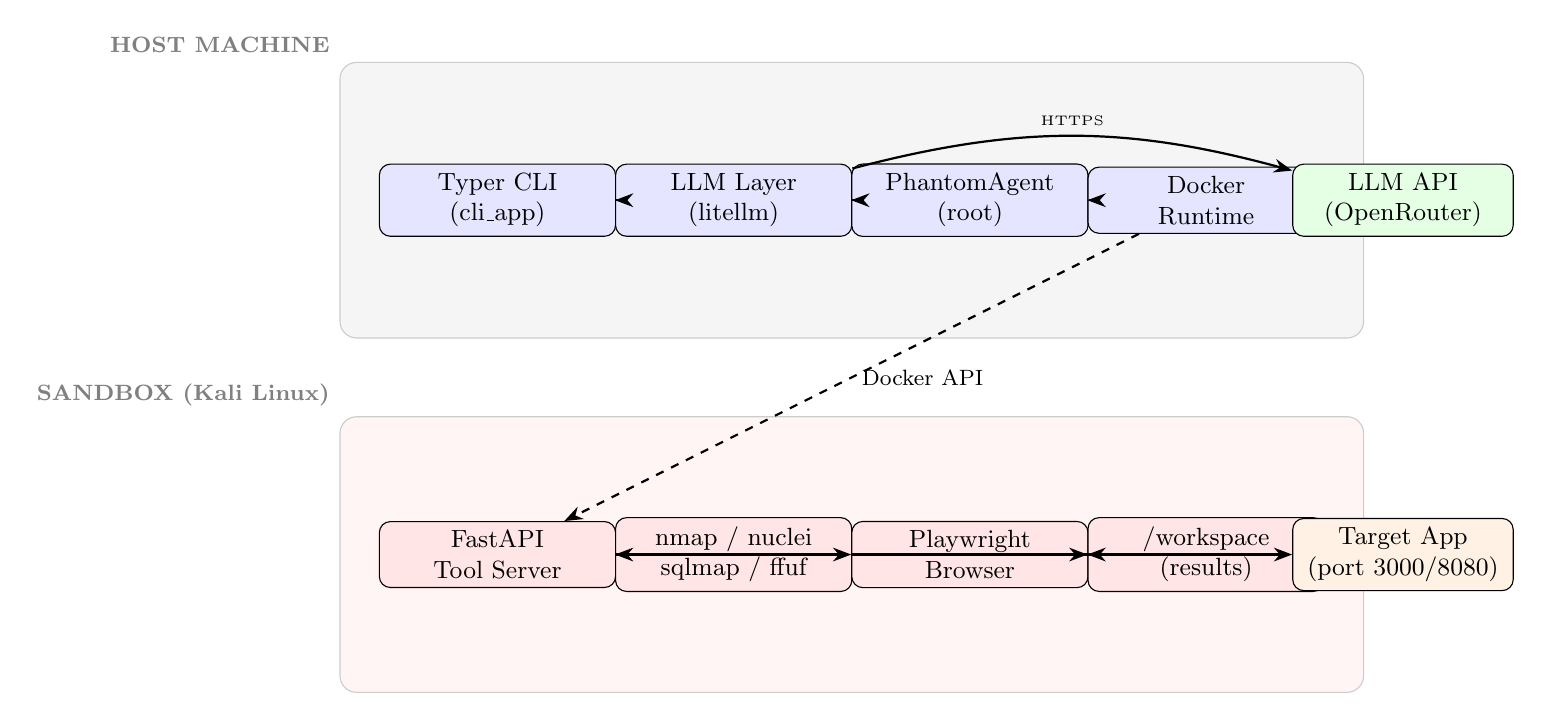
\begin{tikzpicture}[
  box/.style={draw, rounded corners=4pt, minimum width=3cm, minimum height=0.8cm, align=center, font=\small},
  bigbox/.style={draw, rounded corners=6pt, dashed, inner sep=8pt},
  arrow/.style={->, >=Stealth, thick},
  layer/.style={fill=gray!8, draw=gray!40, rounded corners=6pt, inner sep=10pt}
]

% HOST LAYER
\node[layer, minimum width=13cm, minimum height=3.5cm] (host) at (0, 0) {};
\node[above left, font=\footnotesize\bfseries\color{gray}] at (host.north west) {HOST MACHINE};

\node[box, fill=blue!10] (cli) at (-4.5, 0) {Typer CLI\\(cli\_app)};
\node[box, fill=blue!10] (llm) at (-1.5, 0) {LLM Layer\\(litellm)};
\node[box, fill=blue!10] (agent) at (1.5, 0) {PhantomAgent\\(root)};
\node[box, fill=blue!10] (runtime) at (4.5, 0) {Docker\\Runtime};

\draw[arrow] (cli) -- (llm);
\draw[arrow] (llm) -- (agent);
\draw[arrow] (agent) -- (runtime);

% SANDBOX LAYER
\node[layer, minimum width=13cm, minimum height=3.5cm, fill=red!4] (sandbox) at (0, -4.5) {};
\node[above left, font=\footnotesize\bfseries\color{gray}] at (sandbox.north west) {SANDBOX (Kali Linux)};

\node[box, fill=red!10] (api) at (-4.5, -4.5) {FastAPI\\Tool Server};
\node[box, fill=red!10] (tools) at (-1.5, -4.5) {nmap / nuclei\\sqlmap / ffuf};
\node[box, fill=red!10] (browser) at (1.5, -4.5) {Playwright\\Browser};
\node[box, fill=red!10] (ws) at (4.5, -4.5) {/workspace\\(results)};

\draw[arrow] (api) -- (tools);
\draw[arrow] (api) -- (browser);
\draw[arrow] (tools) -- (ws);
\draw[arrow] (browser) -- (ws);

% Docker API connection
\draw[arrow, dashed] (runtime) -- node[right, font=\footnotesize]{Docker API} (api);

% External LLM API
\node[box, fill=green!10, minimum width=2.8cm] (llmapi) at (7, 0) {LLM API\\(OpenRouter)};
\draw[arrow, bend left=15] (llm) to node[above, font=\tiny]{HTTPS} (llmapi);

% Target
\node[box, fill=orange!10, minimum width=2.8cm] (target) at (7, -4.5) {Target App\\(port 3000/8080)};
\draw[arrow] (tools) -- (target);

\end{tikzpicture}
\caption{High-level system architecture of Phantom}
\label{fig:arch}
\end{figure}

\subsection{Component Inventory}

\begin{table}[H]
\centering
\caption{Core Components and Responsibilities}
\begin{tabular}{lll}
\toprule
\textbf{Component} & \textbf{Module} & \textbf{Responsibility} \\
\midrule
CLI & \texttt{phantom.interface.cli\_app} & Typer user interface \\
TUI & \texttt{phantom.interface.tui} & Real-time Textual dashboard \\
LLM Client & \texttt{phantom.llm.llm} & LiteLLM, streaming, retries \\
Memory Compressor & \texttt{phantom.llm.memory\_compressor} & Context window management \\
Agent & \texttt{phantom.agents.PhantomAgent} & Root agent + Jinja2 prompt \\
Tool Executor & \texttt{phantom.tools.executor} & JSON-RPC dispatch \\
Docker Runtime & \texttt{phantom.runtime.docker\_runtime} & Container lifecycle \\
Knowledge Store & \texttt{phantom.core.knowledge\_store} & Thread-safe findings store \\
Audit Logger & \texttt{phantom.core.audit\_logger} & Append-only audit trail \\
Report Generator & \texttt{phantom.core.report\_generator} & Multi-format output \\
SARIF Formatter & \texttt{phantom.interface.formatters.sarif\_formatter} & SARIF 2.1.0 output \\
\bottomrule
\end{tabular}
\end{table}



% ============================================================
\section{Agent Design \& Multi-Agent Protocol}
% ============================================================

\subsection{System Prompt Engineering}

The agent's behavior is fully specified by a Jinja2 system prompt that enforces strict operating rules:

\begin{lstlisting}[caption={System prompt constraints (abbreviated)}]
OPERATING RULES:
1. Every response MUST be a tool call (no plain text)
2. One tool call per response - no speculative multi-step
3. VALIDATE ALL findings with PoC before reporting
4. Never ask for confirmation - work fully autonomously
5. Create specialized sub-agents for each vulnerability class
\end{lstlisting}

The prompt uses \textbf{skill injection} --- domain-specific knowledge blocks are loaded from Markdown files (\texttt{sqli.md}, \texttt{xss.md}, etc.) and embedded at runtime.

\subsection{Tree-Structured Agent Spawning}

\begin{figure}[H]
\centering
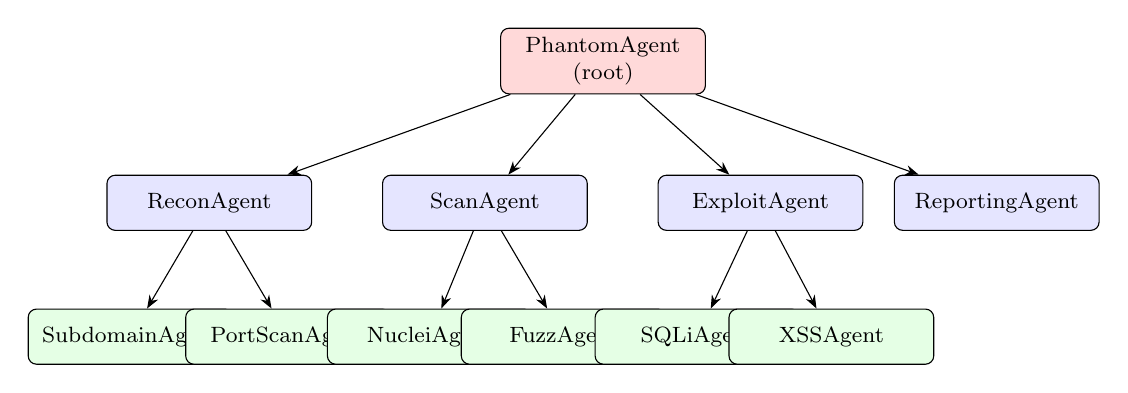
\begin{tikzpicture}[
  agent/.style={draw, rounded corners=3pt, minimum width=2.6cm, minimum height=0.7cm, align=center, font=\footnotesize},
  arrow/.style={->, >=Stealth, thin}
]
\node[agent, fill=red!15] (root) at (0, 0) {PhantomAgent\\(root)};

\node[agent, fill=blue!10] (recon) at (-5, -1.8) {ReconAgent};
\node[agent, fill=blue!10] (scan) at (-1.5, -1.8) {ScanAgent};
\node[agent, fill=blue!10] (exploit) at (2, -1.8) {ExploitAgent};
\node[agent, fill=blue!10] (report) at (5, -1.8) {ReportingAgent};

\draw[arrow] (root) -- (recon);
\draw[arrow] (root) -- (scan);
\draw[arrow] (root) -- (exploit);
\draw[arrow] (root) -- (report);

\node[agent, fill=green!10] (sub) at (-6, -3.5) {SubdomainAgent};
\node[agent, fill=green!10] (port) at (-4, -3.5) {PortScanAgent};
\node[agent, fill=green!10] (nuc) at (-2.2, -3.5) {NucleiAgent};
\node[agent, fill=green!10] (fuzz) at (-0.5, -3.5) {FuzzAgent};
\node[agent, fill=green!10] (sqli) at (1.2, -3.5) {SQLiAgent};
\node[agent, fill=green!10] (xss) at (2.9, -3.5) {XSSAgent};

\draw[arrow] (recon) -- (sub);
\draw[arrow] (recon) -- (port);
\draw[arrow] (scan) -- (nuc);
\draw[arrow] (scan) -- (fuzz);
\draw[arrow] (exploit) -- (sqli);
\draw[arrow] (exploit) -- (xss);
\end{tikzpicture}
\caption{Tree-structured agent spawning hierarchy}
\label{fig:agents}
\end{figure}

\subsection{Agent State Machine}

Enhanced agent state tracks the full scan lifecycle through eight states:

\begin{center}
\texttt{IDLE} $\rightarrow$ \texttt{PLANNING} $\rightarrow$ \texttt{RECONNAISSANCE} $\rightarrow$ \texttt{SCANNING}\\
$\rightarrow$ \texttt{EXPLOITING} $\rightarrow$ \texttt{VERIFYING} $\rightarrow$ \texttt{REPORTING} $\rightarrow$ \texttt{COMPLETE}
\end{center}

All state transitions are protected by a reentrant lock (\texttt{RLock}) ensuring thread safety when sub-agents run in parallel.



% ============================================================
\section{LLM Integration Layer}
% ============================================================

\subsection{Provider-Agnostic Design via LiteLLM}

Phantom uses \textbf{LiteLLM} as a universal abstraction layer:

\begin{lstlisting}[language=bash, caption={Model selection examples}]
PHANTOM_LLM=groq/llama-3.3-70b-versatile
PHANTOM_LLM=openai/gpt-4o
PHANTOM_LLM=openrouter/google/gemma-3-27b-it:free
PHANTOM_LLM=anthropic/claude-sonnet-4-20250514
PHANTOM_LLM=ollama/llama3:70b          # local inference
\end{lstlisting}

\subsection{Supported Providers}

\begin{table}[H]
\centering
\caption{Supported LLM Providers}
\begin{tabular}{lcccc}
\toprule
\textbf{Provider / Model} & \textbf{Free} & \textbf{Vision} & \textbf{Reasoning} & \textbf{Context} \\
\midrule
Groq (Llama 3.3 70B) & \checkmark & -- & -- & 128K \\
OpenRouter (Gemma-3 27B) & \checkmark & -- & -- & 8K \\
OpenRouter (Llama 3.3 70B) & \checkmark & -- & -- & 131K \\
OpenRouter (DeepSeek V3) & \checkmark & -- & -- & 164K \\
OpenAI GPT-4o & -- & \checkmark & -- & 128K \\
Anthropic Claude Sonnet 4 & -- & \checkmark & \checkmark & 200K \\
Google Gemini 2.5 Flash & -- & \checkmark & -- & 1M \\
Ollama (local) & \checkmark & -- & -- & 128K \\
\bottomrule
\end{tabular}
\end{table}

\subsection{Fallback Chain \& Key Rotation}

\begin{lstlisting}[language=bash]
# Primary + fallback providers
PHANTOM_LLM=openai/gpt-4o
PHANTOM_LLM_FALLBACK=groq/llama-3.3-70b-versatile,openrouter/google/gemma-3-27b-it:free

# Round-robin across multiple API keys
LLM_API_KEY=key1,key2,key3,key4
\end{lstlisting}

The \texttt{FallbackChain} advances to the next provider on HTTP 429, 500, 502, or 503 errors. Multi-key rotation uses $i = \text{request\_count} \bmod \text{len(keys)}$ for uniform distribution.

\subsection{Memory Compression}

When conversation history exceeds 100,000 tokens, \texttt{MemoryCompressor} summarizes older messages using the same LLM, preserving:

\begin{itemize}
  \item All confirmed vulnerabilities (id, endpoint, payload);
  \item Technical details (URLs, parameters, authentication tokens);
  \item Failed exploit attempts (prevents duplicate work);
  \item The 15 most recent messages verbatim (recency bias).
\end{itemize}

\subsection{Token Budget Enforcement}

\begin{table}[H]
\centering
\caption{Token Budget Strategy per Provider}
\begin{tabular}{lll}
\toprule
\textbf{Provider} & \textbf{Limit} & \textbf{Strategy} \\
\midrule
Groq free & 5,500 tokens/req & Hard cap (Groq enforces 6K) \\
Small models ($\leq$16K context) & 75\% of context & Conservative trim \\
All others & 85\% of context & Standard trim \\
\bottomrule
\end{tabular}
\end{table}

Messages are trimmed from the \emph{front} (oldest first), permanently preserving the system prompt.



% ============================================================
\section{Security Tool Orchestration}
% ============================================================

\subsection{Tool Invocation Protocol}

The LLM generates tool calls as structured XML:

\begin{lstlisting}[caption={Tool call format}]
<function=run_terminal>
<parameter=command>nmap -sV -sC -p 80,443 192.168.1.1</parameter>
<parameter=timeout>120</parameter>
</function>
\end{lstlisting}

The \texttt{ArgumentParser} extracts parameters, coerces types, and dispatches to the Docker tool server via HTTP POST.

\subsection{Tool Categories}

\begin{table}[H]
\centering
\caption{Available Tools by Category}
\begin{tabular}{lll}
\toprule
\textbf{Category} & \textbf{Tools} & \textbf{Purpose} \\
\midrule
Terminal & \texttt{run\_terminal} & Arbitrary shell execution \\
Security & Nmap, Nuclei, sqlmap, ffuf, Subfinder, Httpx & Scanner wrappers \\
Browser & Playwright-based & JavaScript rendering \\
Proxy & mitmproxy integration & HTTP intercept / replay \\
Python & IPython kernel & Custom exploit scripts \\
File & Read/write sandbox files & Manage wordlists, results \\
Web Search & Perplexity API & Real-time CVE lookup \\
Reporting & \texttt{create\_vulnerability\_report} & Structured finding submission \\
Agents Graph & \texttt{spawn\_agent} & Create sub-agents \\
Finish & \texttt{finish} & Signal scan completion \\
\bottomrule
\end{tabular}
\end{table}

\subsection{Out-of-Band Detection (Interactsh)}

For blind vulnerabilities (blind SSRF, blind XSS, blind SQLi), Phantom integrates \textbf{Interactsh}:

\begin{enumerate}
  \item Register a unique callback URL (\texttt{*.oast.online});
  \item Inject the URL into the payload;
  \item Poll for DNS/HTTP interactions from the target server;
  \item A received interaction \emph{confirms} the vulnerability out-of-band.
\end{enumerate}



% ============================================================
\section{Knowledge Representation}
% ============================================================

\subsection{Vulnerability Model (Pydantic V2)}

The core data model captures the full lifecycle of a finding:

\begin{lstlisting}[language=Python, caption={Vulnerability Pydantic model (abbreviated)}]
class Vulnerability(BaseModel):
    id: str                     # vuln-{sha256[:12]}
    name: str
    vulnerability_class: str    # sqli, xss, rce, ssrf, idor...
    severity: VulnerabilitySeverity
    status: VulnerabilityStatus # detected/verified/exploited
    cvss_score: float | None    # CVSS v3.1, 0.0-10.0
    target: str
    endpoint: str | None
    parameter: str | None
    payload: str | None         # Working PoC payload
    evidence: list[VulnerabilityEvidence]
    cve_ids: list[str]
    cwe_ids: list[str]
    remediation: str | None
    detected_at: datetime
    verified_at: datetime | None
\end{lstlisting}

\subsection{CVSS Severity Mapping}

Phantom computes CVSS v3.1 scores using the \texttt{cvss} library and maps them to severity levels:

\begin{table}[H]
\centering
\caption{CVSS Score to Severity Mapping}
\begin{tabular}{lll}
\toprule
\textbf{CVSS Score} & \textbf{Severity} & \textbf{Color Code} \\
\midrule
9.0--10.0 & \textcolor{criticalred}{\textbf{Critical}} & Red \\
7.0--8.9 & \textcolor{highorange}{\textbf{High}} & Orange \\
4.0--6.9 & \textcolor{mediumyellow}{\textbf{Medium}} & Yellow \\
0.1--3.9 & \textcolor{lowgreen}{\textbf{Low}} & Green \\
0.0 & Informational & Gray \\
\bottomrule
\end{tabular}
\end{table}

\subsection{MITRE ATT\&CK Enrichment}

All findings are automatically annotated with ATT\&CK for Enterprise:

\begin{table}[H]
\centering
\caption{Vulnerability to ATT\&CK Technique Mapping}
\begin{tabular}{ll}
\toprule
\textbf{Vulnerability Class} & \textbf{MITRE Technique} \\
\midrule
SQL Injection & T1190 (Exploit Public-Facing Application) \\
XSS / CSRF & T1059 (Command and Scripting Interpreter) \\
SSRF & T1083 (File \& Directory Discovery) + T1041 (Exfiltration) \\
Weak Authentication & T1110 (Brute Force) + T1078 (Valid Accounts) \\
IDOR & T1530 (Data from Cloud Storage) \\
\bottomrule
\end{tabular}
\end{table}

\subsection{Compliance Mapping}

\begin{table}[H]
\centering
\caption{Compliance Framework Cross-Reference}
\begin{tabular}{lllll}
\toprule
\textbf{Vulnerability} & \textbf{PCI-DSS} & \textbf{GDPR} & \textbf{OWASP Top 10} & \textbf{CWE} \\
\midrule
SQL Injection & 6.3 & Art.\,32 & A03:2021 & CWE-89 \\
XSS & 6.3 & Art.\,32 & A03:2021 & CWE-79 \\
Broken Authentication & 8.2 & Art.\,32 & A07:2021 & CWE-287 \\
IDOR & 6.3 & Art.\,5 & A01:2021 & CWE-639 \\
SSRF & 6.6 & Art.\,32 & A10:2021 & CWE-918 \\
\bottomrule
\end{tabular}
\end{table}



% ============================================================
\section{Sandboxed Execution Environment}
% ============================================================

\subsection{Container Configuration}

The sandbox is a Kali Linux Docker container with:

\begin{itemize}
  \item \textbf{Base image}: \texttt{kalilinux/kali-rolling}
  \item \textbf{Installed tools}: nmap, nuclei, sqlmap, ffuf, subfinder, httpx, gospider, katana, arjun, jwt\_tool, wafw00f, interactsh-client, Playwright (headless Chrome)
  \item \textbf{User}: \texttt{pentester} (sudo NOPASSWD)
  \item \textbf{Python}: Poetry venv with FastAPI, IPython
  \item \textbf{Workspace}: \texttt{/workspace} (persisted via Docker bind mount)
\end{itemize}

\subsection{Tool Server API}

\begin{lstlisting}[caption={Tool server REST endpoints (FastAPI)}]
POST /tools/run_terminal     -> Execute shell command + return stdout/stderr
POST /tools/browser/navigate -> Playwright navigation
POST /tools/proxy/start      -> Start mitmproxy intercept
POST /tools/python/execute   -> Run in IPython kernel
GET  /health                 -> Container readiness probe
\end{lstlisting}

\subsection{Security Boundaries}

\begin{table}[H]
\centering
\caption{Security Isolation Boundaries}
\begin{tabular}{ll}
\toprule
\textbf{Boundary} & \textbf{Implementation} \\
\midrule
Process isolation & Docker namespaces + cgroups \\
Filesystem isolation & Container FS; bind mount for \texttt{/workspace} only \\
Scope validation & \texttt{ScopeValidator} blocks out-of-scope targets \\
Audit trail & \texttt{AuditLogger}: every tool call logged (append-only) \\
No destructive actions & Enforced by system prompt + scope validator \\
\bottomrule
\end{tabular}
\end{table}



% ============================================================
\section{Reporting \& Output Formats}
% ============================================================

\subsection{Output Format Overview}

\begin{table}[H]
\centering
\caption{Supported Report Formats}
\begin{tabular}{llp{7cm}}
\toprule
\textbf{Format} & \textbf{Flag} & \textbf{Use Case} \\
\midrule
JSON & \texttt{--output-format json} & Machine-readable; full technical detail \\
SARIF 2.1.0 & \texttt{--output-format sarif} & GitHub Advanced Security, GitLab SAST \\
Markdown & \texttt{--output-format markdown} & Human-readable; briefings, tickets \\
HTML & \texttt{--output-format html} & Self-contained web report with severity badges \\
\bottomrule
\end{tabular}
\end{table}

\subsection{SARIF 2.1.0 CI/CD Integration}

The SARIF formatter produces schema-compliant output for GitHub Advanced Security:

\begin{lstlisting}[language=yaml, caption={GitHub Actions integration}]
- name: Run Phantom
  run: |
    docker run --rm \
      -e PHANTOM_LLM=openrouter/google/gemma-3-27b-it:free \
      -e LLM_API_KEY=${{ secrets.OPENROUTER_KEY }} \
      redwan07/phantom:latest \
      scan -t $TARGET_URL --output-format sarif

- name: Upload SARIF
  uses: github/codeql-action/upload-sarif@v3
  with:
    sarif_file: phantom_runs/report.sarif.json
\end{lstlisting}



% ============================================================
\section{Evaluation \& Testing}
% ============================================================

\subsection{Test Suite}

Phantom ships with \textbf{146 unit and integration tests}, all passing as of v0.8.0:

\begin{table}[H]
\centering
\caption{Test Coverage by Category}
\begin{tabular}{lrc}
\toprule
\textbf{Test Category} & \textbf{Count} & \textbf{Pass Rate} \\
\midrule
Module imports & 25 & 100\% \\
Config loading / persistence & 12 & 100\% \\
LLM response parsing & 18 & 100\% \\
Vulnerability models & 20 & 100\% \\
Tool argument parsing & 42 & 100\% \\
Scope validation & 8 & 100\% \\
SARIF formatting & 8 & 100\% \\
Memory compressor & 7 & 100\% \\
Agent state transitions & 6 & 100\% \\
\midrule
\textbf{Total} & \textbf{146} & \textbf{100\%} \\
\bottomrule
\end{tabular}
\end{table}

\subsection{External User Audit}

A systematic external-user audit was conducted in February 2026. The repo was cloned from GitHub and tested as a first-time user. \textbf{11 defects were identified and fixed}:

\begin{table}[H]
\centering
\caption{Bugs Found and Fixed in External Audit}
\begin{tabular}{rp{5cm}lp{4.5cm}}
\toprule
\textbf{\#} & \textbf{Bug} & \textbf{Severity} & \textbf{Fix Applied} \\
\midrule
1 & \texttt{\_convert\_to\_bool("")} raises \texttt{ValueError} & High & Return \texttt{bool(value)} fallback \\
2 & Same for \texttt{\_convert\_to\_bool("text")} & High & Same fix \\
3--5 & Pydantic V2 \texttt{json\_encoders} deprecated & Low & Migrate to \texttt{@field\_serializer} \\
6 & \texttt{pytest addopts} includes \texttt{--cov} flags & Medium & Remove from defaults \\
7 & \texttt{typer[all]} extra removed in typer 0.15 & Low & Remove extras pragma \\
8 & SARIF URL pointed to old org & Low & Update to \texttt{Usta0x001/Phantom} \\
9 & Sandbox image URL inaccessible & High & Update to \texttt{redwan07/phantom:latest} \\
10 & Markdown/HTML export were stubs & Medium & Full implementation \\
11 & OpenRouter absent from provider presets & Medium & Added 6 presets \\
\bottomrule
\end{tabular}
\end{table}

\noindent\textbf{Result}: 144/146 → 146/146 tests passing.

\subsection{OWASP Juice Shop Benchmark}

OWASP Juice Shop is the standard benchmark for web application security testing tools, containing 100+ intentional vulnerabilities across all OWASP Top 10 categories~\cite{juiceshop}.

\begin{table}[H]
\centering
\caption{Expected OWASP Top 10 Coverage by Phantom}
\begin{tabular}{clc}
\toprule
\textbf{Category} & \textbf{Description} & \textbf{Coverage} \\
\midrule
A01:2021 & Broken Access Control & \checkmark \\
A02:2021 & Cryptographic Failures & \checkmark \\
A03:2021 & Injection (SQLi, XSS, ...) & \checkmark \\
A04:2021 & Insecure Design & \checkmark \\
A05:2021 & Security Misconfiguration & \checkmark \\
A06:2021 & Vulnerable Components & \checkmark \\
A07:2021 & Identification \& Auth Failures & \checkmark \\
A08:2021 & Software \& Data Integrity & -- \\
A09:2021 & Security Logging Failures & \checkmark \\
A10:2021 & Server-Side Request Forgery & \checkmark \\
\bottomrule
\end{tabular}
\end{table}



% ============================================================
\section{Security \& Ethical Considerations}
% ============================================================

\subsection{Authorization Requirement}

Running Phantom against systems without explicit written permission is illegal in most jurisdictions (e.g., CFAA in the US, EU Directive 2013/40/EU on attacks against information systems). The tool requires explicit user confirmation of authorization before any scan begins.

\subsection{Scope Validation}

The \texttt{ScopeValidator} component enforces boundaries at the tool-call level. Any URL, IP address, or hostname not matching the authorized target set raises \texttt{OutOfScopeError} — blocking the tool call before it reaches the sandbox.

\subsection{No-Destructive-Action Policy}

The system prompt prohibits:

\begin{itemize}
  \item Data deletion or modification;
  \item Denial-of-Service or resource exhaustion attacks;
  \item Credential stuffing beyond authorized scope;
  \item Lateral movement to out-of-scope hosts.
\end{itemize}

\subsection{Audit Trail}

Every tool call is persisted in an append-only \texttt{AuditLogger}:

\begin{lstlisting}[language=Python, caption={Audit log entry structure}]
{
  "timestamp": "2026-02-23T12:00:00Z",
  "agent_id": "agent-abc123",
  "tool": "run_terminal",
  "args": {"command": "nmap -sV target.com"},
  "result_hash": "sha256:...",
  "session_id": "scan-xyz"
}
\end{lstlisting}

\subsection{Data Privacy}

No scan data is sent to external telemetry services. API keys are stored at \texttt{\textasciitilde/.phantom/cli-config.json} with Unix permissions \texttt{0600}.



% ============================================================
\section{Conclusion \& Future Work}
% ============================================================

\subsection{Summary}

Phantom demonstrates that a carefully designed LLM orchestration framework, combined with professional security tooling, can perform effective autonomous penetration testing. Key achievements:

\begin{enumerate}
  \item \textbf{Full autonomy}: Zero human interaction from scan start to report delivery;
  \item \textbf{Multi-agent scalability}: Tree-structured spawning enables parallel specialization;
  \item \textbf{Provider flexibility}: 15+ LLM providers including free-tier options;
  \item \textbf{Standards compliance}: SARIF 2.1.0, CVSS 3.1, CWE, MITRE ATT\&CK;
  \item \textbf{Production quality}: Docker distribution, 146-test suite, structured audit logging.
\end{enumerate}

\subsection{Limitations}

\begin{table}[H]
\centering
\caption{Current Limitations and Planned Mitigations}
\begin{tabular}{p{4cm}p{4.5cm}p{4.5cm}}
\toprule
\textbf{Limitation} & \textbf{Impact} & \textbf{Planned Fix} \\
\midrule
Full Docker dependency & Cannot run without Docker & Pure Python static analysis mode \\
No authenticated scan (OAuth/SAML) & Misses post-login bugs & OAuth2 flow automation \\
No mobile app analysis & iOS/Android excluded & Appium integration \\
Context window limits on free models & May truncate long sessions & Better memory compression \\
No CI integration tests & Regression risk & GitHub Actions test matrix \\
\bottomrule
\end{tabular}
\end{table}

\subsection{Roadmap}

\begin{description}
  \item[v0.9.0] Authenticated scan flows (session cookies, OAuth2, JWT injection)
  \item[v1.0.0] Continuous monitoring mode (re-scan on code push via webhook)
  \item[v1.1.0] Source code SAST integration (Semgrep + LLM reasoning)
  \item[v1.2.0] Mobile application testing (APK decompilation + API surface testing)
  \item[Long term] Multi-agent adversarial simulation (red vs.\ blue agent competition)
\end{description}



% ============================================================
\section*{References}
\label{sec:references}
\addcontentsline{toc}{section}{References}
% ============================================================

\begin{thebibliography}{99}

\bibitem{isc2024}
ISC2 (2024).
\textit{Cybersecurity Workforce Study 2024}.
\url{https://www.isc2.org/research}

\bibitem{pentestgpt2023}
Deng, G., Liu, Y., Mayoral-Vilches, V., Liu, P., Li, Y., Xu, Y., Zhang, T., Liu, Y., Pinzger, M., \& Rass, S. (2023).
\textit{PentestGPT: An LLM-Empowered Automatic Penetration Testing Tool}.
arXiv:2308.06782.

\bibitem{hackingbuddy2023}
Happe, A. \& Cito, J. (2023).
\textit{Getting pwn'd by AI: Penetration Testing with Large Language Models}.
arXiv:2308.00121.

\bibitem{autoattacker2024}
Xu, Y., et al. (2024).
\textit{AutoAttacker: A Large Language Model Guided System to Implement Automatic Cyber Attacks}.
arXiv:2403.01038.

\bibitem{react2023}
Yao, S., Zhao, J., Yu, D., Du, N., Shafran, I., Narasimhan, K., \& Cao, Y. (2023).
\textit{ReAct: Synergizing Reasoning and Acting in Language Models}.
ICLR 2023. arXiv:2210.03629.

\bibitem{tot2023}
Yao, S., Yu, D., Zhao, J., Shafran, I., Griffiths, T. L., Cao, Y., \& Narasimhan, K. (2023).
\textit{Tree of Thoughts: Deliberate Problem Solving with Large Language Models}.
arXiv:2305.10601.

\bibitem{owasp2021}
OWASP Foundation (2021).
\textit{OWASP Top Ten 2021}.
\url{https://owasp.org/Top10/}

\bibitem{juiceshop}
Bjoern Kimminich (2024).
\textit{OWASP Juice Shop}.
\url{https://github.com/juice-shop/juice-shop}

\bibitem{mitre}
MITRE Corporation (2024).
\textit{MITRE ATT\&CK for Enterprise}.
\url{https://attack.mitre.org/}

\bibitem{cvss}
FIRST.org (2019).
\textit{Common Vulnerability Scoring System (CVSS) v3.1 Specification}.
\url{https://www.first.org/cvss/}

\bibitem{sarif}
OASIS (2020).
\textit{Static Analysis Results Interchange Format (SARIF) Version 2.1.0}.
\url{https://docs.oasis-open.org/sarif/sarif/v2.1.0/}

\bibitem{ptes2014}
PTES Technical Guidelines (2014).
\textit{Penetration Testing Execution Standard}.
\url{http://www.pentest-standard.org/}

\bibitem{litellm}
BerriAI (2024).
\textit{LiteLLM: Universal LLM API}.
\url{https://github.com/BerriAI/litellm}

\end{thebibliography}

% ============================================================
\newpage
\appendix
\section*{Appendix A: CLI Command Reference}
\addcontentsline{toc}{section}{Appendix A: CLI Command Reference}
% ============================================================

\begin{lstlisting}[language=bash, caption={Complete CLI usage}]
# Core scan command
phantom scan -t <target> [options]
  --model, -m       LLM model (overrides PHANTOM_LLM env var)
  --scan-mode       quick | standard | deep (default: standard)
  --instruction, -i Additional instruction for the agent
  --output-format   json | sarif | markdown | html | all
  --non-interactive Run without TUI (for CI/CD)
  --verbose         Print full LLM conversation

# Configuration
phantom config show              # Display current configuration
phantom config set KEY VALUE     # Set a config value
phantom config reset             # Reset to defaults

# Reports
phantom report list              # List past scan reports
phantom report export ID FORMAT  # Export a report in another format
phantom report show ID           # Print report summary

# General
phantom version                  # Print version info
phantom --help                   # Full help text
\end{lstlisting}

% ============================================================
\section*{Appendix B: Environment Variables}
\addcontentsline{toc}{section}{Appendix B: Environment Variables}
% ============================================================

\begin{table}[H]
\centering
\caption{Phantom Environment Variables}
\begin{tabular}{lll}
\toprule
\textbf{Variable} & \textbf{Default} & \textbf{Description} \\
\midrule
\texttt{PHANTOM\_LLM} & -- & Primary LLM model \\
\texttt{LLM\_API\_KEY} & -- & API key(s) (comma-separated for rotation) \\
\texttt{LLM\_API\_BASE} & -- & Custom API base URL \\
\texttt{PHANTOM\_LLM\_FALLBACK} & -- & Comma-separated fallback providers \\
\texttt{PHANTOM\_IMAGE} & \texttt{redwan07/phantom:latest} & Sandbox Docker image \\
\texttt{PHANTOM\_SANDBOX\_TIMEOUT} & \texttt{600} & Max sandbox execution time (s) \\
\texttt{PHANTOM\_SCAN\_MODE} & \texttt{standard} & Default scan depth \\
\texttt{PHANTOM\_OUTPUT\_FORMAT} & \texttt{json} & Default report format \\
\bottomrule
\end{tabular}
\end{table}

\vspace{2cm}
\begin{center}
\rule{0.5\linewidth}{0.4pt}\\[0.3cm]
{\small This report was prepared to document the academic contributions of the Phantom project for coursework submission at ESTIN. All testing was performed against intentionally vulnerable systems (OWASP Juice Shop) or systems with explicit written authorization.}\\[0.3cm]
\textcopyright~2026 Gadouri Redwan --- MIT License
\end{center}

\end{document}
